\section{Experiments}

In this section, we describe the experimental setup and results of our approach. We focus on two key components: (1) the efficient representation of point cloud data using an Octree structure, which enables significant reduction in the number of points while preserving essential information; and (2) the application of Graph Neural Networks (GNNs) for classification tasks on this reduced dataset. We provide a detailed explanation of our experimental methodology, including the minute details of our implementation, and present the results obtained from these experiments.

\subsection{Point Reduction with Octree}\label{ssec:expt_octree}
    \begin{figure}
        \centering
        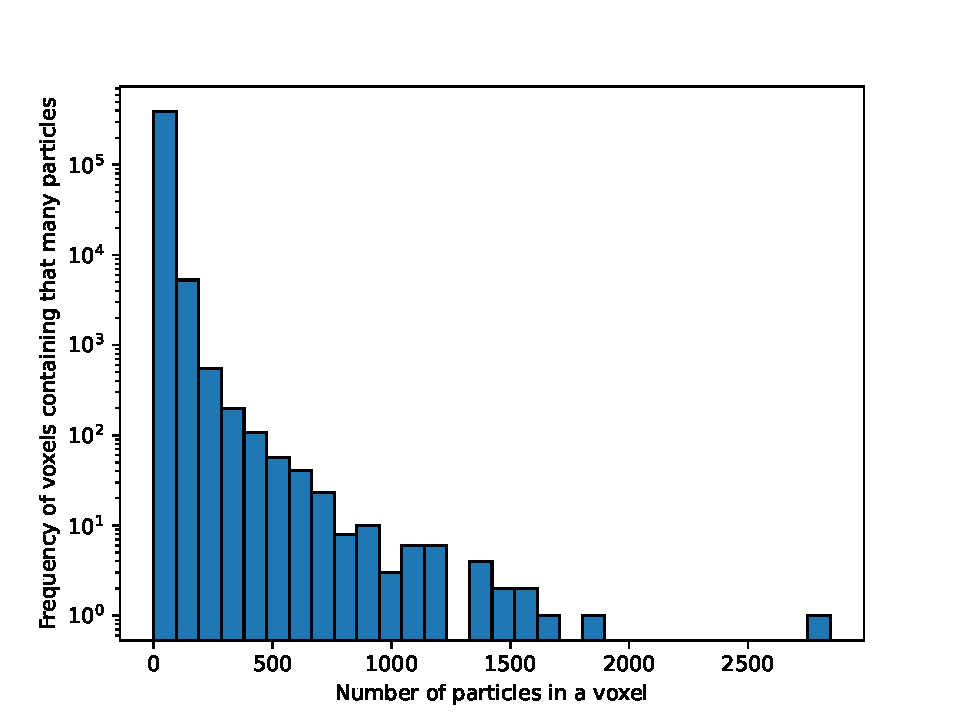
\includegraphics[width=\linewidth]{images/g1.pdf}
        \caption{Log scale frequency plot of masses of the voxels (mass is equivalent to number of particles in that voxel)}
        \label{graph:1}
    \end{figure}

    We worked with the smallest data available on the site for now. The data is available on the website \url{https://www.tng-project.org/data/}. There we took the gravity-only data of the lowest resolution and worked on it. The idea was to develop the algorithm and codes for the lowest one first and then try the bigger data later. So we worked with the data named \texttt{TNG50-4-Dark}. It's simulation volume is 51.7 mega parsec cube and has $270^3$ ($\approx2\times10^7$) particles.

    The first problem was to reduce the number of particles by voxelization. As explained in \ref{ssec:octree} we used the octree algorithm. We initially had $2\times10^7$. There are two tunable parameters in the Octree algorithm: 

    \begin{itemize}
        \item \texttt{max\_particles\_per\_voxel}: This is the upper limit of particles in a voxel. No voxel in principle should carry more than these many points. \textbf{We kept this value to 100.}
        \item \texttt{min\_voxel\_size}: Because this is a recursive algorithm, and that we knew that there are certain locations in the space where the density of particles is tremendously large. So we kept this check that if the voxel size reduces below this point, we would not divide the voxels any further even if it had far more particles than \texttt{max\_particles\_per\_voxel}. \textbf{We kept this value to be 0.001.} This means, the minimum voxel size is 0.001 times the simulation length (which is 51.7 mega parsec here).
    \end{itemize}

    Upon converting the point cloud to octree these are the statistics of the data:

    \begin{itemize}
        \item Total number of voxels: 395286 ($\approx2\%$ of $2\times10^7$)
        \item Number of voxels with less than 100 particles: 388990 (98.4\%)
        \item Number of voxels with more than 100 particles: 6292 (1.6\%)
    \end{itemize}

    Figure \ref{graph:1} shows the log-scaled distribution of a number of particles in voxels.

\subsection{Prediction Using GNN}

    In Figure \ref{graph:eg_halo} he have shown a halo at random. In this halo, we can see that if the background points are somehow removed, it would be really easy to classify the halo points into different halos using naive Machine learning algorithms like \textbf{DB-Scan}. So if we can train a model which can differentiate between the background and the foreground (semantic segmentation task), we can then run clustering algorithms on the foreground to do the instance segmentation task. So the tough problem of instance segmentation got boiled down to classifying the points into background and foregorund.

    \begin{figure}[h]
        \centering
        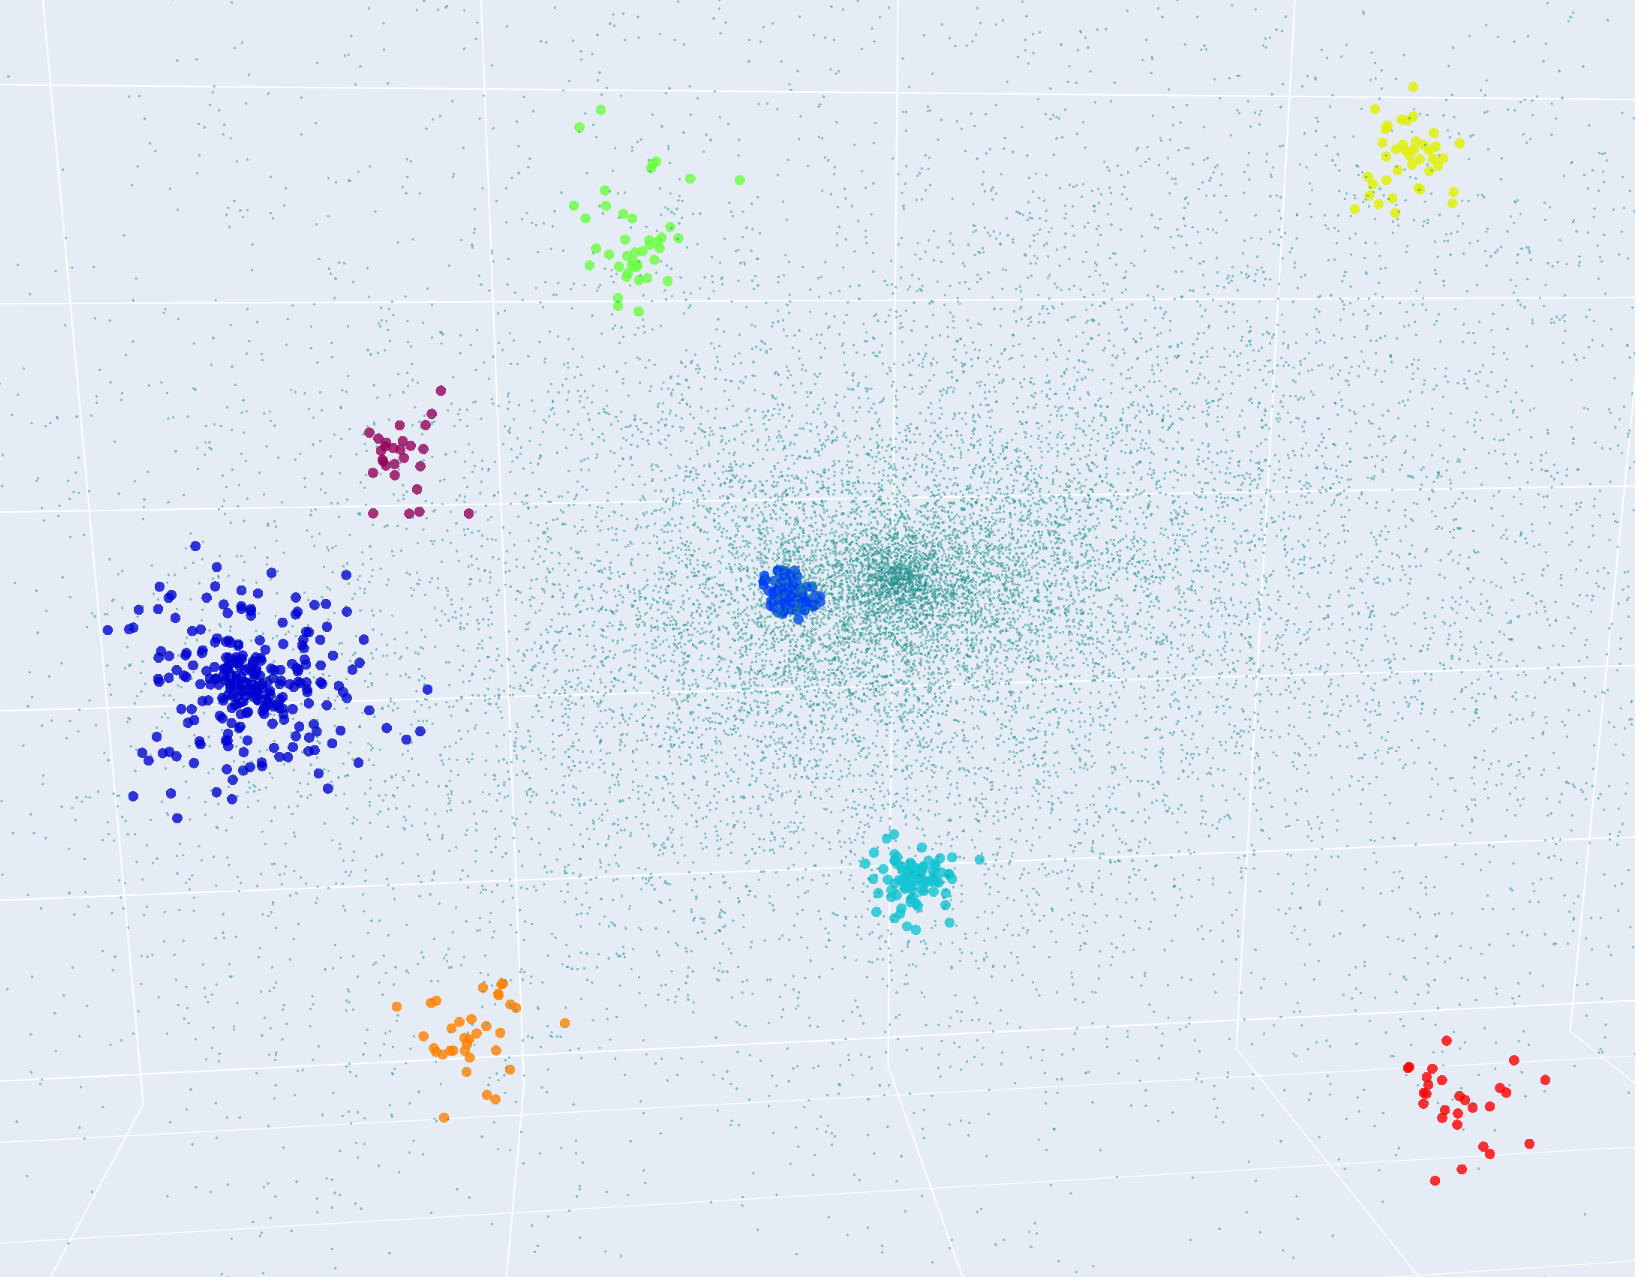
\includegraphics[width=0.9\linewidth]{images/g2.png}
        \caption{Visualizing a halo: The different subhalos have been given different colours, and the background points have been made fine and given dark green colour}
        \label{graph:eg_halo}
    \end{figure}

    \begin{figure}
        \centering
        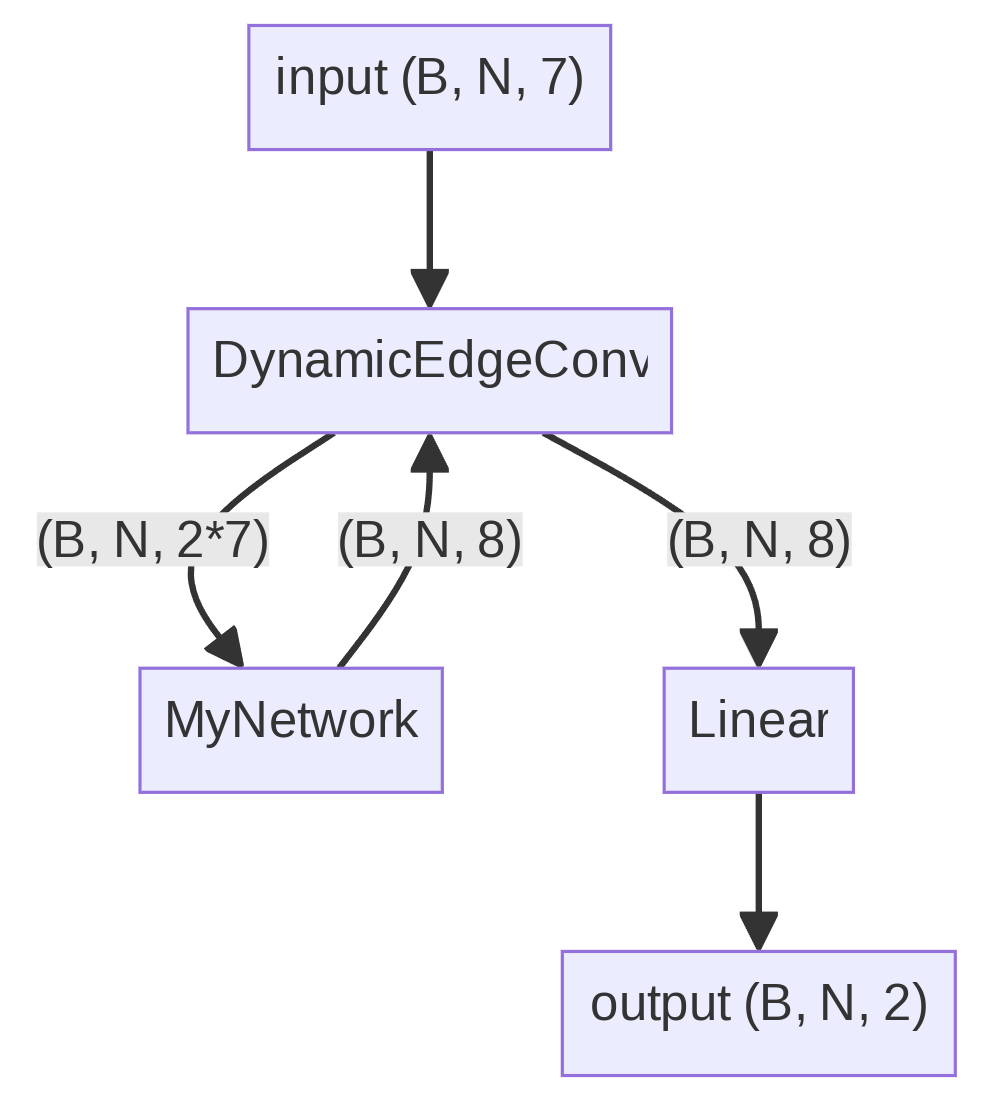
\includegraphics[width=0.9\linewidth]{images/network.png}
        \caption{Architecture of the Used Network}
        \label{fig:network}
    \end{figure}

    \begin{figure}
        \centering
        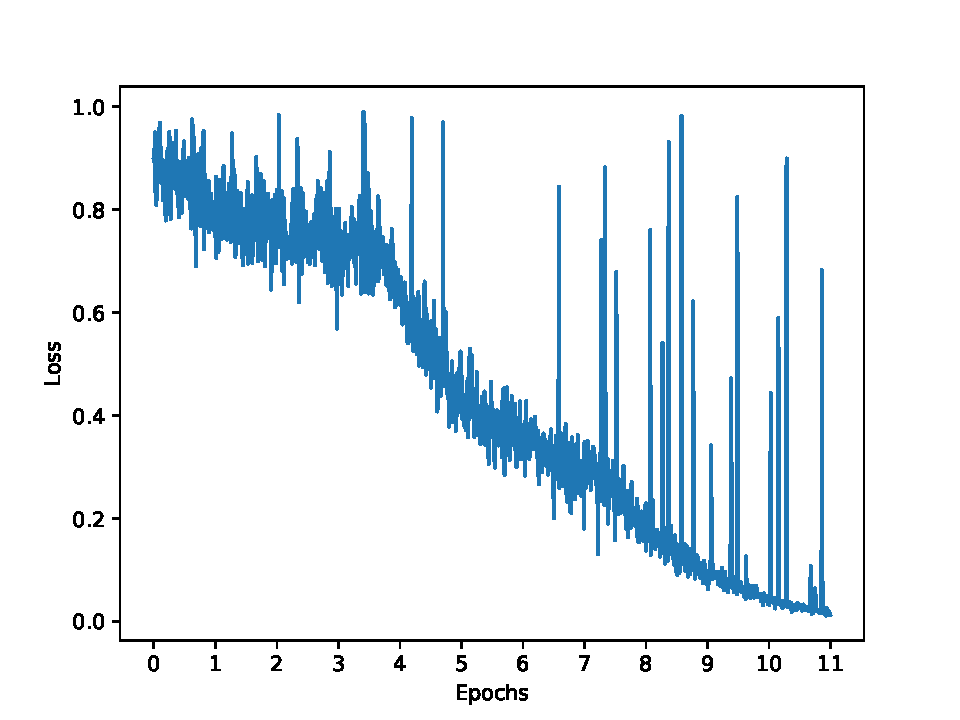
\includegraphics[width=0.9\linewidth]{images/loss.pdf}
        \caption{Decreasing Loss with epoch}
        \label{fig:loss}
    \end{figure}

    The proposed model consists of a Graph Neural Network (GNN) backbone, which leverages a simple Multi-Layer Perceptron (MLP) as its message passing function. This MLP, denoted by $\mathit{MyNetwork}$, is composed of three fully connected layers with ReLU non-linearity in between, specifically $7\times2\rightarrow8\rightarrow8\rightarrow8$. The GNN backbone employs this MLP to update node features during the message passing step, as described in Equation \ref{eq:message}. The output from the GNN backbone is then passed through a final linear layer to produce the ultimate output of the model. The model architecture is given in Figure \ref{fig:network}.
    

    Here we should have predicted the output using clustering algorithms, but I didn't get enough time to do that. So, I am showing how my model is being able to differentiate between the foreground and the background clearly. 

    The model is trained using stochastic gradient descent (SGD) as the optimization algorithm, with a learning rate of $5 \times 10^{-2}$, momentum of 0.95, and weight decay of 0.0001. We used Binary-Crossentropy-Loss as the loss-function. Initially before applying smote, our loss was decreasing, but we were not getting very good results. This was because the data was not balanced, there were far more points in the background class than the foreground. Hence we applied resampling technique called SMOTE (explained in detail in \ref{ssec:smote}). As a result, in figure \ref{fig:loss} we see how the loss function decreases over training, and we also get good results to show (an example is shown is Figure \ref{fig:result})

    \begin{figure}
        \centering
        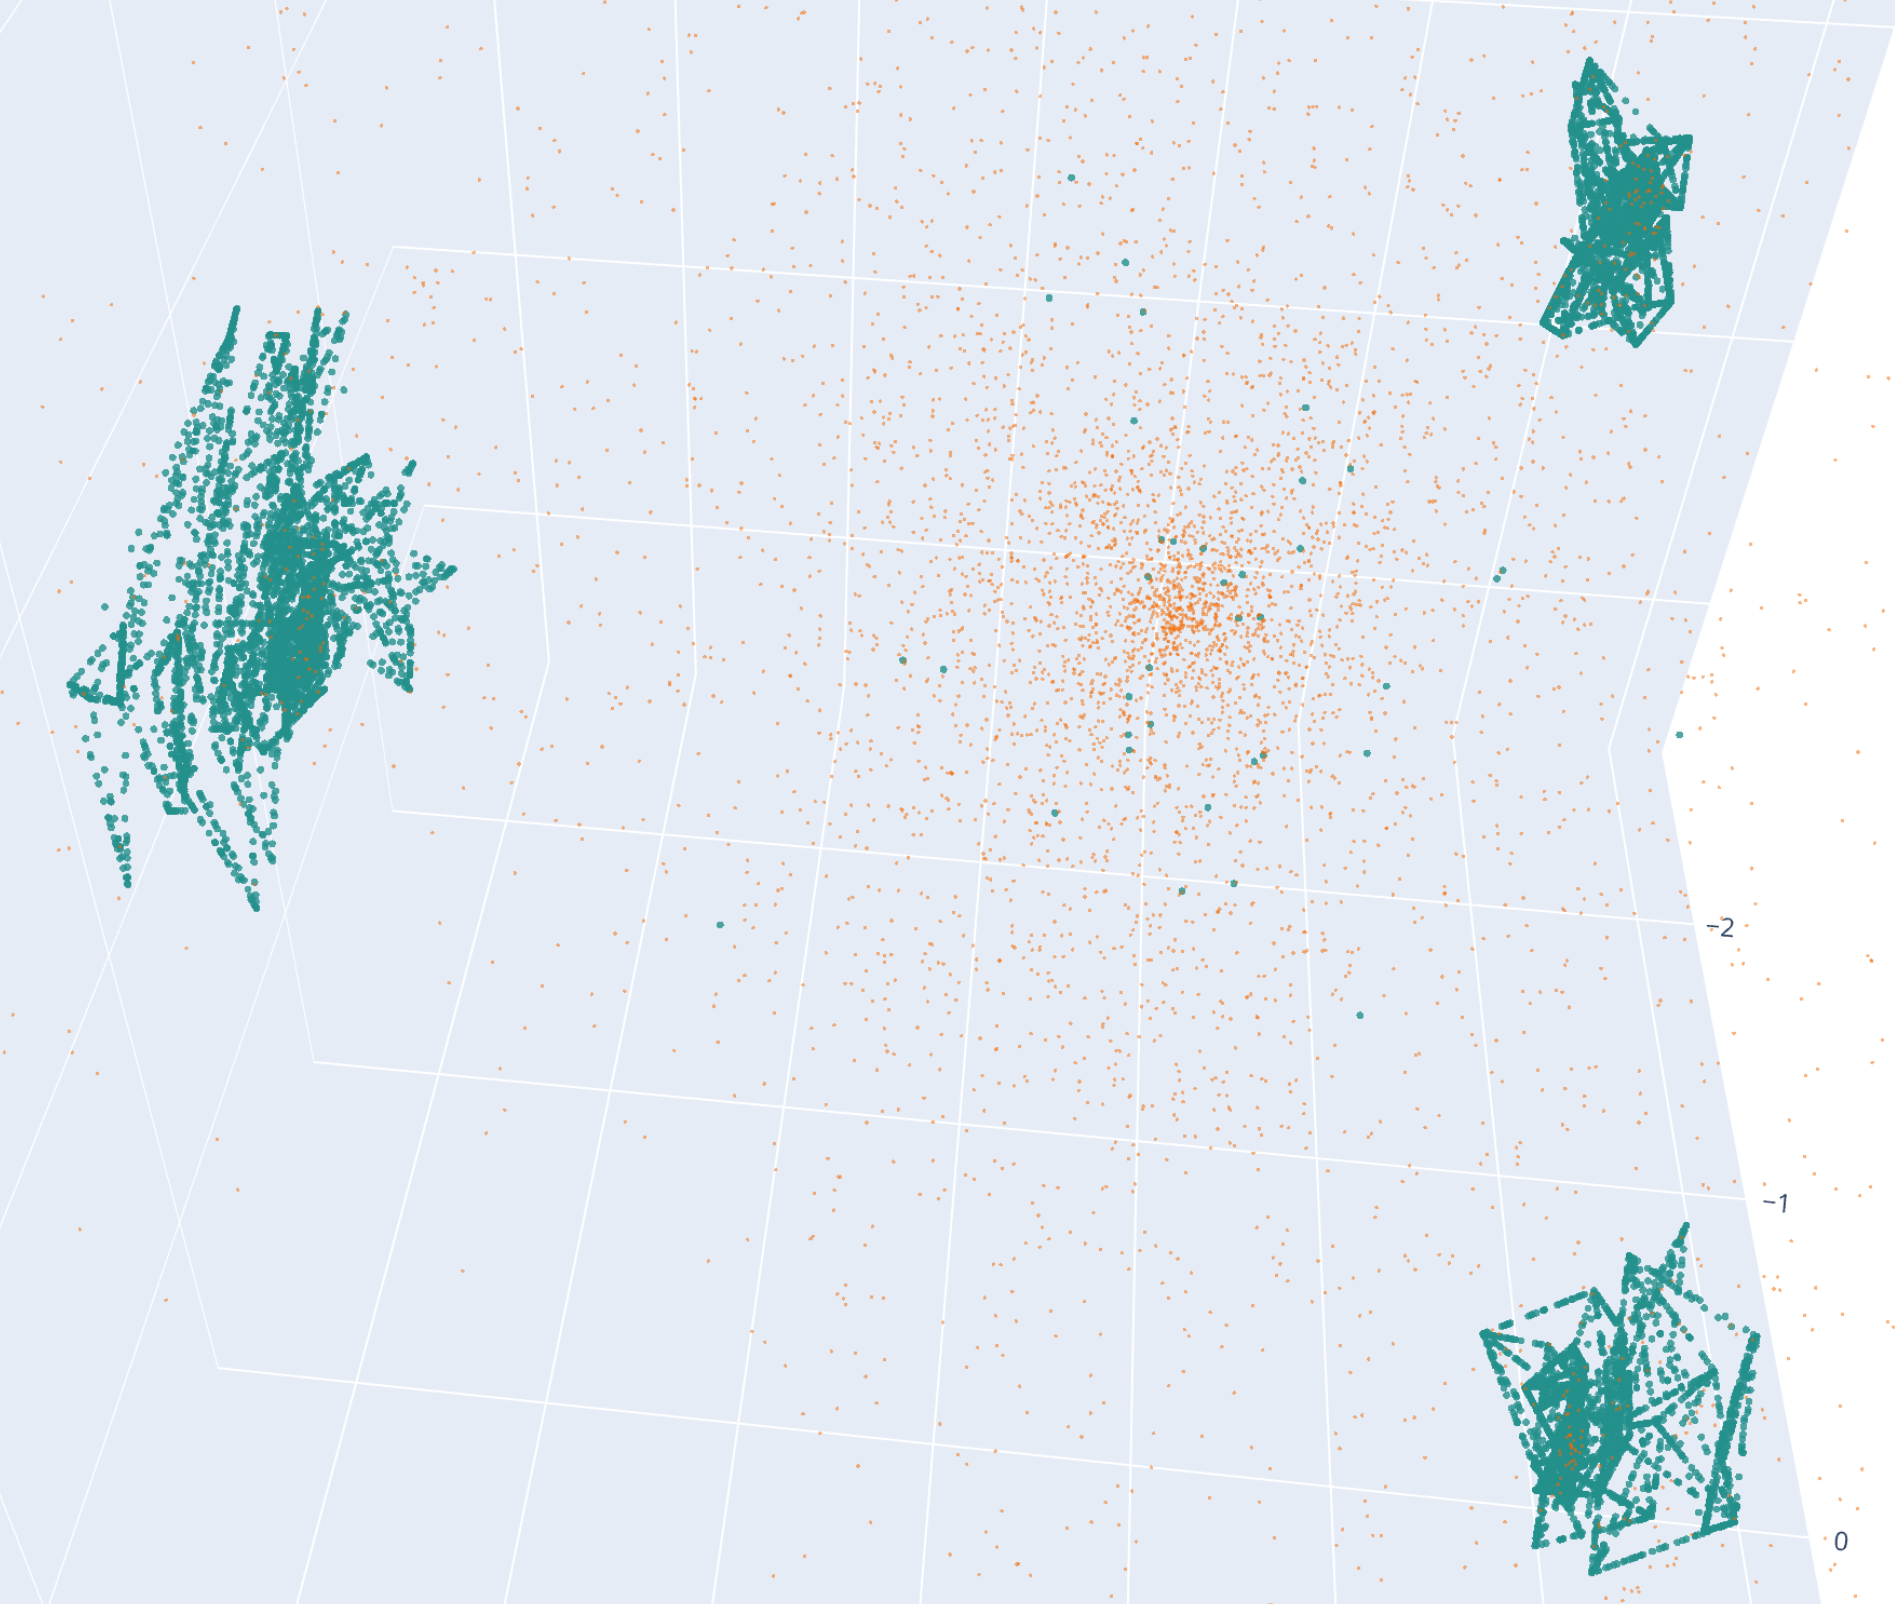
\includegraphics[width=0.9\linewidth]{images/result.png}
        \caption{Example Output From our model (green points have been labelled as foreground and orange points have been labelled as background by model)}
        \label{fig:result}
    \end{figure}
